\section{Yleistä lippukunnasta}
\begin{figure}[htb]
	\begin{center}
		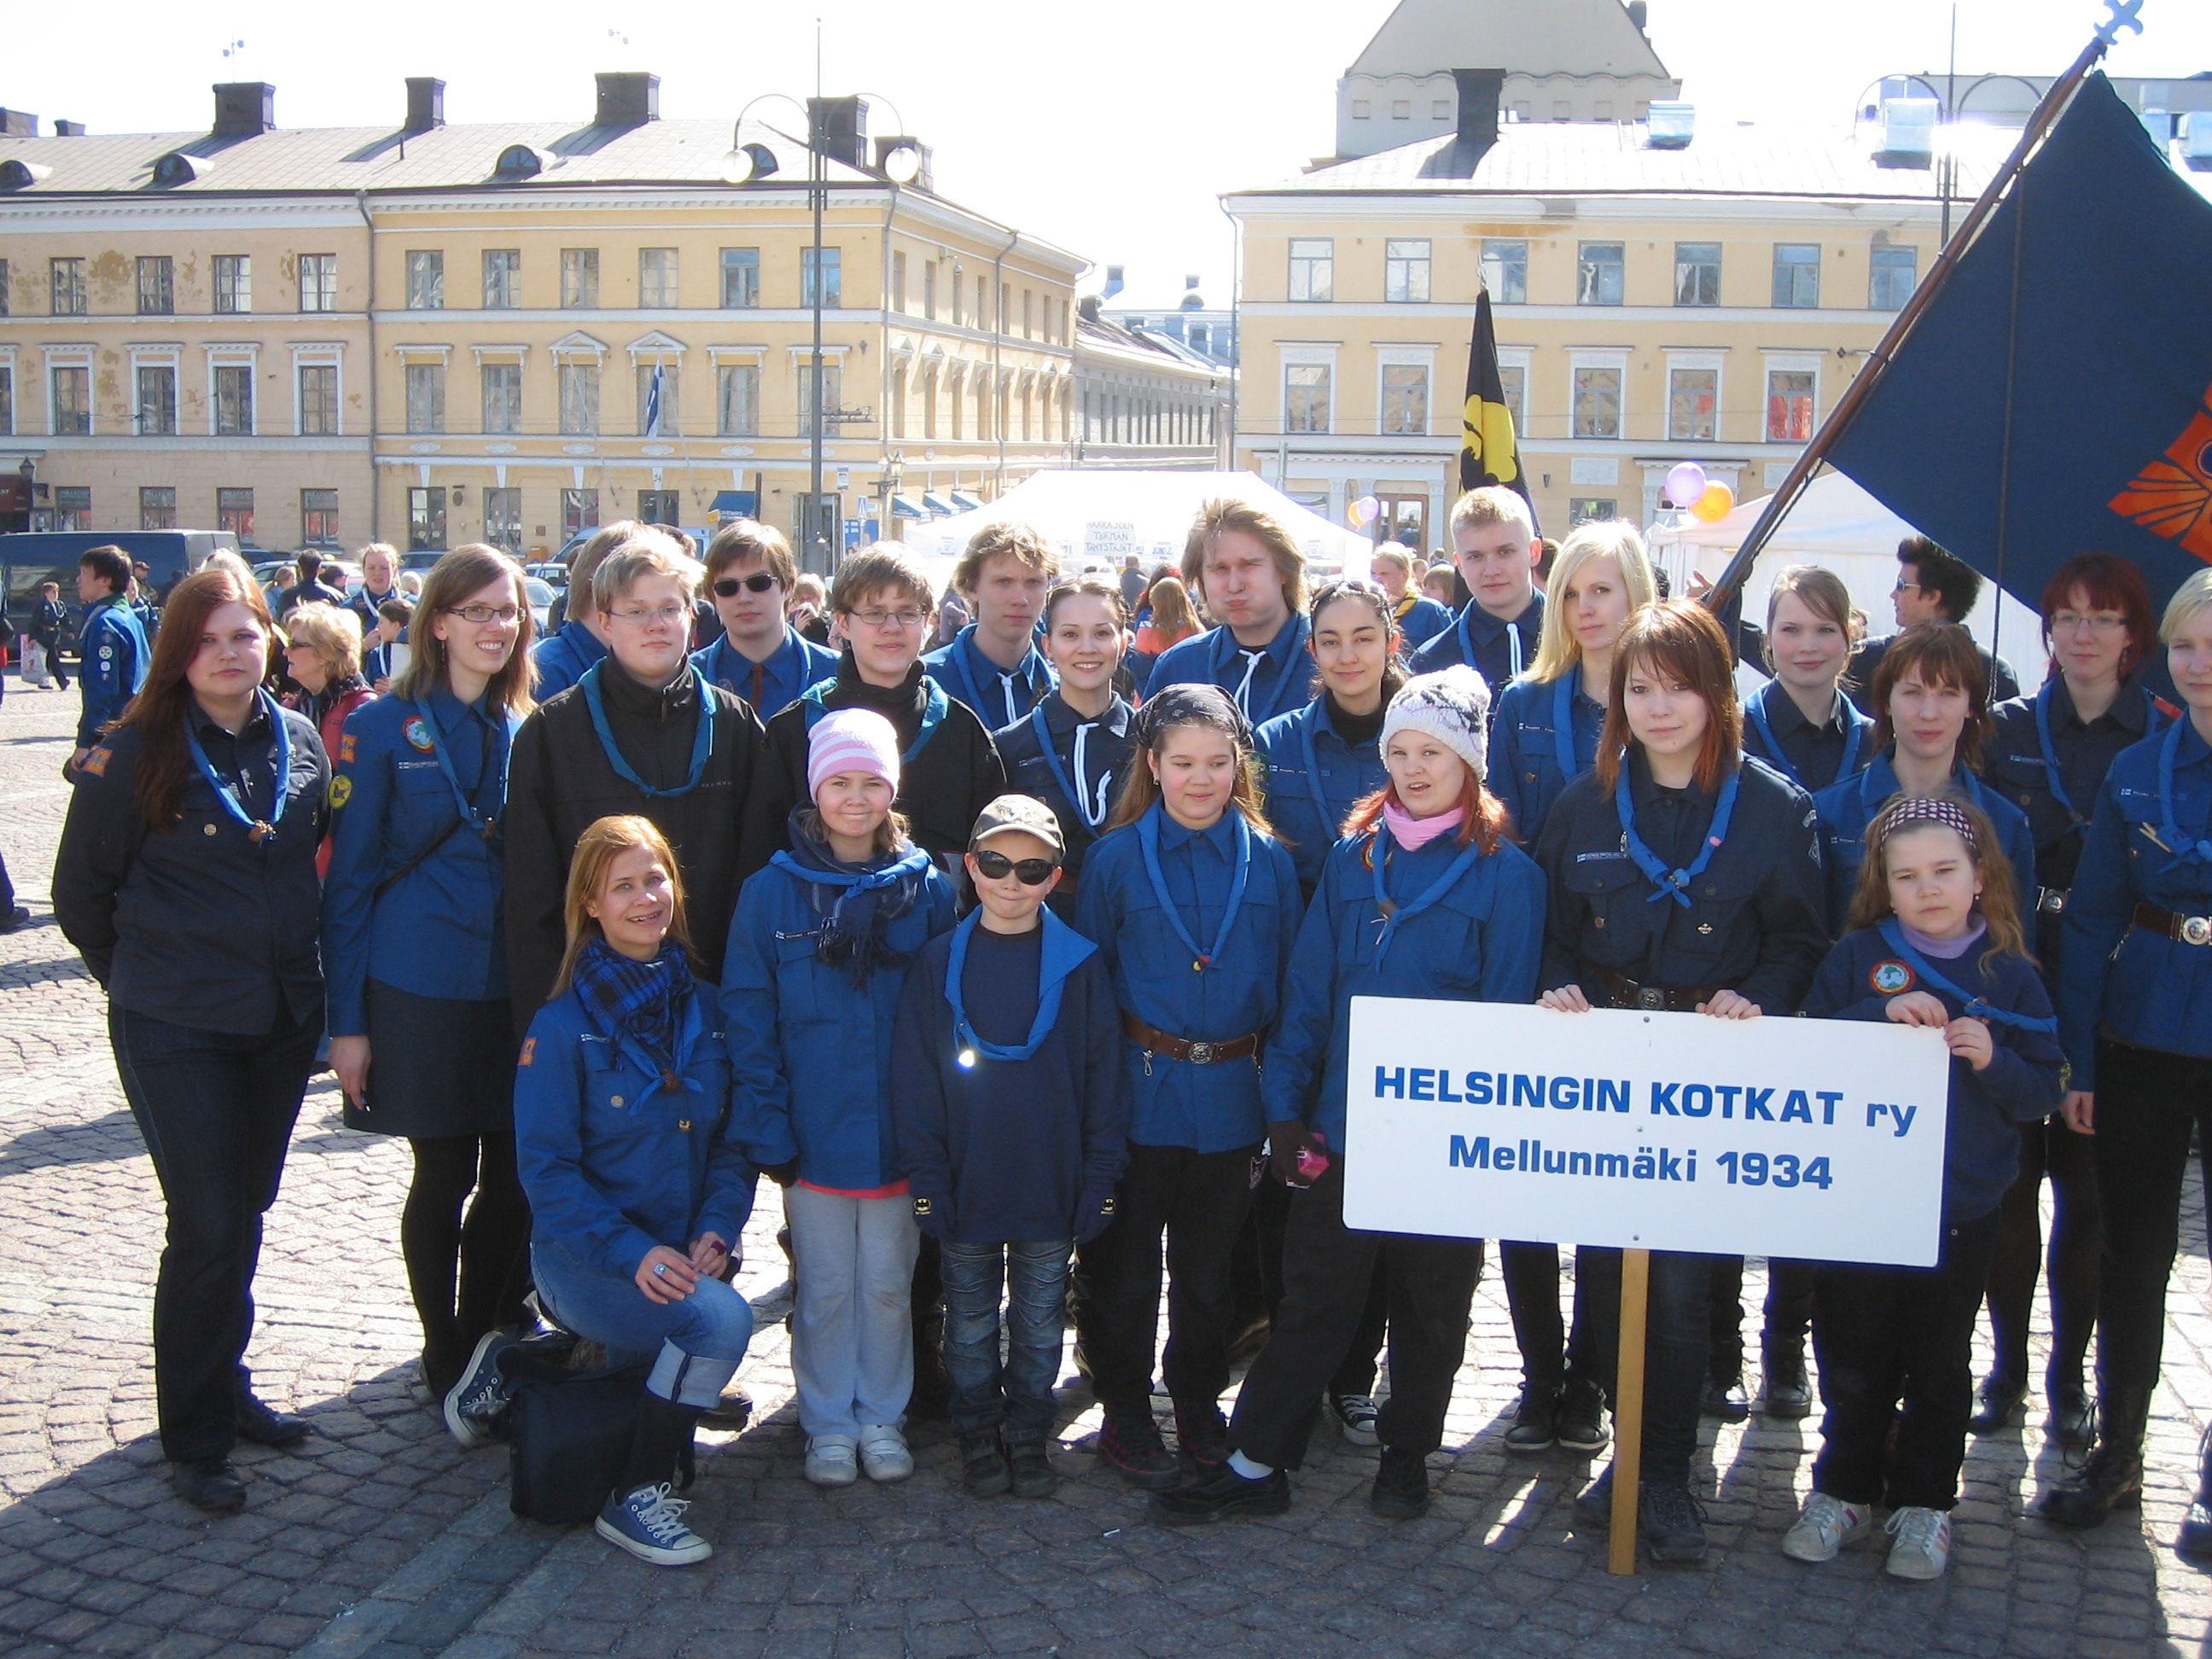
\includegraphics[height=7cm]{kuvat/paraatissa.jpg}
	\end{center}
	\captionsetup{labelformat=empty}
	%\caption{\textbf{Lippukunnan kämppä, Kyöpeli.}}
\end{figure}

Helsingin Kotkat on vuonna 1934 alunperin poikalippukunnaksi Helsingin keskustaan perustettu partiolippukunta. Myöhemmin lippukunta yhdistyi paikallisen tyttölippukunnan kanssa sekalippukunnaksi ja muutti Mellunmäkeen, jossa se toimii edelleen. Lippukunnalla on pitkät perinteet erityisesti luonnossa liikkumisessa ja partiotaitokilpailuissa. Lippukunnan pitkä ikä näkyy toiminnassa ja perinteissä ja vanhatkin, jopa jo eläkkeellä olevat jäsenet toimivat lippukunnassa edelleen aktiivisesti.\\
\\Helsingin Kotkat toteuttaa toiminnassaan Suomen Partiolaisten partio-ohjelmaa. Toiminta oli kuluneella kaudella aktiivista ja lippukunnan jäsenmäärä oli vakaa. Lippukunta osallistui aktiivisesti läheisten lippukuntien kanssa järjestettyyn yhteistoimintaan ja oli kantava voima kaupunginosansa nuorisötyössä.\\
\\Lippukunnassa toimi keväällä 2016 yksi tyttösudenpentulauma, kaksi poikasudenpentulaumaa, yksi tyttöseikkailijajoukkue, yksi poikatarpojajoukkue, yksi tyttötarpojaryhmä sekä yksi poikasamoajaryhmä. Lisäksi lippukunnan johtajatehtävisä toimivat vaeltajat ja aikuiset ovat kokoontuneet toiminnansuunnittelun merkeissä. Myös johtajahuoltoa järjestettiin, jotta johtajiston jaksaminen saatiin taattua. 
\newpage

